\section{Subset Extraction}

In Quicksort, we partition our input into two sets: those smaller than the 
pivot, and those larger or equal. The situation in Quickhull is more similar
to the Dutch National Flag Problem, with the following three options for each
point: belonging in $S_1$, in $S_2$, or neither. The key difference is that
we do not need to preserve the points belonging in neither. We extract two
subsets, but these do not have to be a partition.
This allows us to modify the more efficient algorithms for bipartitioning.

\subsection{Sequential Extraction}

It is possible to vectorize the partitioning of Quicksort using a compress
instruction that is in the AVX-512 instruction set \cite{Bramas17},
or with a portable software implementation of this instruction \cite{Blacher22}.
This is done by reading a vector of values from either the left or right of the
array, partitioning this vector in registers, and then writing it back to the
front and back of the array. During this process, the invariant of 
Figure~\ref{fig:invariant_bramas} is maintained.

\begin{figure}[ht]
    \resizebox{\columnwidth}{!}{%
        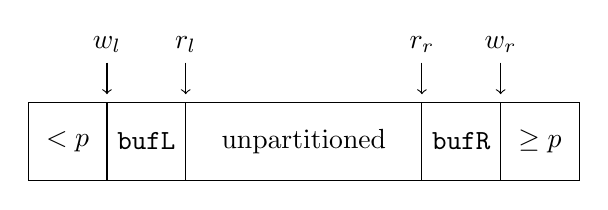
\begin{tikzpicture}
            \draw (0, 0) rectangle (1, 1) node[midway] {$< p$};
            \draw (1, 0) rectangle (2, 1) node[midway] {\texttt{bufL}};
            \draw (2, 0) rectangle (5, 1) node[midway] {unpartitioned};
            \draw (5, 0) rectangle (6, 1) node[midway] {\texttt{bufR}};
            \draw (6, 0) rectangle (7, 1) node[midway] {$\geq p$};

            \draw[->] (1, 1.5) node[above] {$w_l$} -- (1, 1.1);
            \draw[->] (2, 1.5) node[above] {$r_l$} -- (2, 1.1);
            \draw[->] (5, 1.5) node[above] {$r_r$} -- (5, 1.1);
            \draw[->] (6, 1.5) node[above] {$w_r$} -- (6, 1.1);
        \end{tikzpicture}
    }
    \caption{Invariant for partitioning an array into values smaller than
             a pivot $p$ and larger or equal than $p$. The values in
             \texttt{bufL}, \texttt{bufR} are buffered and can be safely
             overwritten. A write and a read pointer are maintained for
             the left and right side of the array.}
    \label{fig:invariant_bramas}
\end{figure}

Let $d$ be the number of element fitting in a vector register. The invariant
is started with \texttt{bufL} and \texttt{bufR} having space of at least
$d$ elements. As we read and write $d$ elements per iteration, the sum
of $r_l - w_l$ and $w_r - r_r$ stays $2d$, ensuring that at least one side
has enough space to write $d$ elements to.

There is enough space on the left whenever

\begin{equation}
(r_l - w_l) \geq d \iff r_l - w_l \geq 2d - (r_l - w_l) \iff r_l - w_l \geq w_r - r_r.
\label{eq:bramas}
\end{equation}

In this case there is already enough space on the left, so we take this as
condition to read $d$ elements from the right. Analogously, there is enough
space of the right when this condition does not hold.

We use almost the same algorithm: we write points belonging in $S_1$ to the
left, and points in $S_2$ to the right. As we may write back less than
$d$ elements, we get some undefined parts of the array as illustrated in
Figure~\ref{fig:invariant_qhull}.

\begin{figure}[ht]
    \resizebox{\columnwidth}{!}{%
        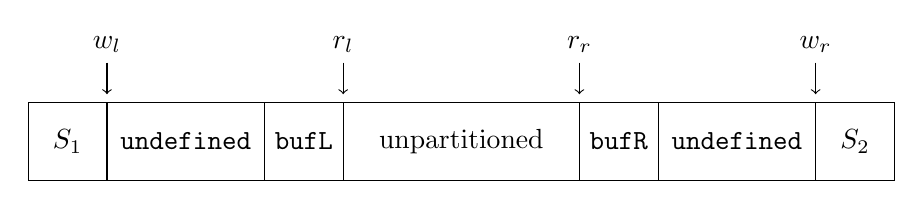
\begin{tikzpicture}
            \draw (0, 0)  rectangle (1, 1)  node[midway] {$S_1$};
            \draw (1, 0)  rectangle (3, 1)  node[midway] {\texttt{undefined}};
            \draw (3, 0)  rectangle (4, 1)  node[midway] {\texttt{bufL}};
            \draw (4, 0)  rectangle (7, 1)  node[midway] {unpartitioned};
            \draw (7, 0)  rectangle (8, 1)  node[midway] {\texttt{bufR}};
            \draw (8, 0)  rectangle (10, 1) node[midway] {\texttt{undefined}};
            \draw (10, 0) rectangle (11, 1) node[midway] {$S_2$};

            \draw[->] (1,  1.5)  node[above] {$w_l$} -- (1,  1.1);
            \draw[->] (4,  1.5)  node[above] {$r_l$} -- (4,  1.1);
            \draw[->] (7,  1.5)  node[above] {$r_r$} -- (7,  1.1);
            \draw[->] (10, 1.5)  node[above] {$w_r$} -- (10, 1.1);
        \end{tikzpicture}
    }
    \caption{Invariant for partitioning a set of points $P$ into 
             $S_1$ and $S_2$ as described in 
             Algorithm~\ref{alg:quickhull_basic}. 
             The values in \texttt{bufL}, \texttt{bufR}
             are buffered and can be safely overwritten. The values marked
             as undefined are not buffered and can be safely overwritten.
             A write and a read pointer are maintained for
             the left and right side of the array.}
    \label{fig:invariant_qhull}
\end{figure}

As $(r_l - w_l) + (w_r - r_r) \geq 2d$, the inequalities of 
Equation~\ref{eq:bramas} hold in our case as well.

\subsection{Parallel Extraction}

Partitioning has linear complexity, so it is very likely to be limited by
bandwidth. For this reason, minimizing data-movement is the primary design goal
of the parallel algorithm. The algorithm consists out of two conceptual steps:
a parallel step where each thread works on a subset of $P$ local to it, and 
a sequential cleanup step. This approach is inspired by \cite{francis92}.

\subsubsection{Local Extraction}

We first divide the points over the threads in a block-cyclic distribution.
(Figure~\ref{fig:blockcycl}) according to some block parameter $b$.

\begin{figure}[ht]
    \resizebox{\columnwidth}{!}{%
        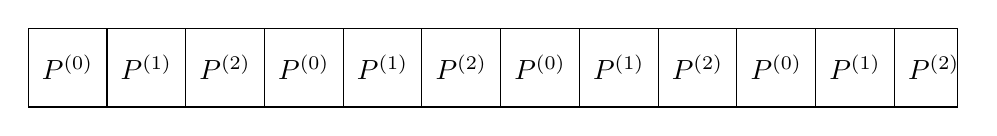
\begin{tikzpicture}
            \foreach \i in {0, ..., 10} {
                \draw (\i, 0) rectangle (\i + 1, 1);
            }
            \draw (11, 0) rectangle (11.8, 1);

            \foreach \i in {0, ..., 3} {
                \node at (3 * \i + 0.5, 0.5) {$P^{(0)}$};
            }
            \foreach \i in {0, ..., 3} {
                \node at (3 * \i + 1.5, 0.5) {$P^{(1)}$};
            }
            \foreach \i in {0, ..., 3} {
                \node at (3 * \i + 2.5, 0.5) {$P^{(2)}$};
            }
        \end{tikzpicture}
    }
    \caption{Block cyclic distribution over $3$ threads. Each square represents
             $b$ elements, except the last one that may contain less.}
    \label{fig:blockcycl}
\end{figure}

To be more precise, given $n$ points total and $n_t$ threads, we partition
the index set $I = [0, n)$ into

$$I^{(t)} = \{t \cdot b + l \cdot n_t \cdot b + j \ | \ 0 \leq j < b,
                0 \leq t \cdot b + l \cdot n_t \cdot b + j < n\}$$

for $t = 0, \cdots, n_t - 1$. Thread $t$ can then work on its subset
$P^{(t)} := \{P[i] \ | \ i \in I^{(t)}\}$ independently from the other threads.

We have each thread extract the subsets from its $P^{(t)}$ in parallel, 
returning $c_{1}^{(t)}, c_{2}^{(t)} \in I^{(t)}$ such that
$\{P[i] \ | \ i \in I^{(t)}, i < c^{(t)}\} \subseteq S_1$
and $\{P[i] \ | \ i \in I^{(t)}, c^{(t)} \leq i\} \subseteq S_2$.
Denoting $c_{l}^{\min / \max}$ for the minimum / maximum of $c_1$, $c_2$, this
gives us a permuted $P$ where indices in $[0, c_1^{min})$ belong to $S_1$,
indices in $[c_{1}^{\max}, c_2^{\min})$ are in $(S_1 \cup S_2)^c$, and
indices in $[c_2^{\max}, n)$ are in $S_2$, as depicted in 
Figure~\ref{fig:local_part}.

The key observation is that for random $P$ and $n_t, b \ll n$, the ratio 
$|S_1| : |S_2|$ is roughly equal to $|S_1 \cap P^{(t)}| : |S_2 \cap P^{(t)}|$.
This means that the $c_1^{(t)}$s are expected to be close to each other, and
the global $c_1$, and likewise for the $c_2^{(t)}$s. This even holds for $P$
not random, but already a convex hull listed in clockwise, or counter-clockwise
order. As it is not performance-critical, a naive Dutch National Flag Algorithm 
suffices for permuting $[c_1^{min}, c_1^{\max}) \cup [c_2^{min}, c_2^{\max})$.

\begin{figure}[ht]
    \resizebox{\columnwidth}{!}{%
        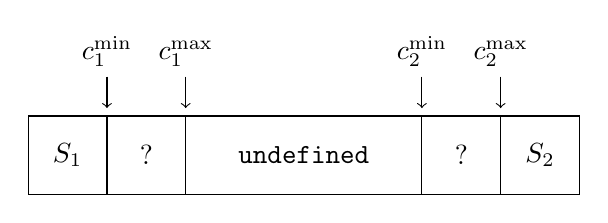
\begin{tikzpicture}
            \draw (0, 0) rectangle (1, 1) node[midway] {$S_1$};
            \draw (1, 0) rectangle (2, 1) node[midway] {$?$};
            \draw (2, 0) rectangle (5, 1) node[midway] {$\texttt{undefined}$};
            \draw (5, 0) rectangle (6, 1) node[midway] {$?$};
            \draw (6, 0) rectangle (7, 1) node[midway] {$S_2$};

            \draw[->] (1, 1.5) node[above] {$c_1^{\min}$} -- (1, 1.1);
            \draw[->] (2, 1.5) node[above] {$c_1^{\max}$} -- (2, 1.1);
            \draw[->] (5, 1.5) node[above] {$c_2^{\min}$} -- (5, 1.1);
            \draw[->] (6, 1.5) node[above] {$c_2^{\max}$} -- (6, 1.1);
        \end{tikzpicture}
    }
    \caption{The points $P$ after local partition. The points in $?$ can
             belong to either $S_1$, $S_2$, or can be undefined.}
    \label{fig:local_part}
\end{figure}

\subsubsection{Cleanup}

\tkcomment{TODO: Jordy}

Writes to and from RAM are done in aligned chunks, typically $64$ bytes, called
cachelines. This makes it expensive for different processors to write to the 
same cacheline. To avoid this problem we make $b$ a multiple of
the cacheline size, and cut off some points at the start to ensure proper
alignment. The distance between $c_i^{min}$ and $c_i^{max}$ is proportional
to $b$, so we cannot choose it too large. However, loading a vector register 
from non-contiguous data is expensive and this can occur around the boundary
of blocks. So $b$ should not be too small either. We found $b = 2048$ a good
compromise.
